\documentclass{beamer}
\usepackage{color}
\usepackage[english]{babel}
\usepackage[utf8]{inputenc}
\usepackage{times}
\usepackage[T1]{fontenc}

\mode<presentation>
{
  \usetheme{CambridgeUS}

  \useoutertheme{infolines}
  % \useoutertheme{shadow}
  \useinnertheme{circles}

  \setbeamertemplate{footline}
  {
    \leavevmode%
    \hbox{%
    \begin{beamercolorbox}[wd=.333333\paperwidth,ht=2.25ex,dp=1ex,center]{author in head/foot}%
      \usebeamerfont{author in head/foot}\insertshortauthor
    \end{beamercolorbox}%
    \begin{beamercolorbox}[wd=.333333\paperwidth,ht=2.25ex,dp=1ex,center]{title in head/foot}%
      \usebeamerfont{title in head/foot}Master Thesis
    \end{beamercolorbox}%
    \begin{beamercolorbox}[wd=.333333\paperwidth,ht=2.25ex,dp=1ex,right]{date in head/foot}%
      \insertframenumber{} / \inserttotalframenumber\hspace*{2ex}
    \end{beamercolorbox}}%
    \vskip0pt%
  }

  \setbeamertemplate{navigation symbols}{}
}

\title{Content-Based Image Retrieval}
\author{Léo Vetter}
\date{November 9, 2015}

\institute[Passau University and INSA Lyon] % (optiobnal, but mostly needed)
{
  \inst{1}%
  Department of Computer Science\\
  University of Passau
  \and
  \inst{2}%
  IT Department\\
  INSA Lyon}

\subject{Theoretical Computer Science}

% If you have a file called "university-logo-filename.xxx", where xxx
% is a graphic format that can be processed by latex or pdflatex,
% resp., then you can add a logo as follows:

% \pgfdeclareimage[height=0.5cm]{university-logo}{university-logo-filename}
% \logo{\pgfuseimage{university-logo}}

\AtBeginSection[]
{
  \begin{frame}<beamer>{Outline}
    \tableofcontents[currentsection,currentsubsection]
  \end{frame}
}

\begin{document}

\begin{frame}
  \titlepage
\end{frame}

\begin{frame}{Outline}
  \tableofcontents
  % You might wish to add the option [pausesections]
\end{frame}

\section{Content-Based Image Retrieval}

  \subsection{Definition}

    \begin{frame}{Definition}

      \begin{columns}[c]
        \column{.5\textwidth} % column designated by a command
        \begin{center}
          {\color{green} Yes}
        \end{center}
        \begin{figure}
          
\includegraphics[width=0.6\textwidth]{images/slides/image.png}
        \end{figure}
        \column{.5\textwidth}
        \begin{center}
          {\color{red} No}
        \end{center}
        \begin{figure}
          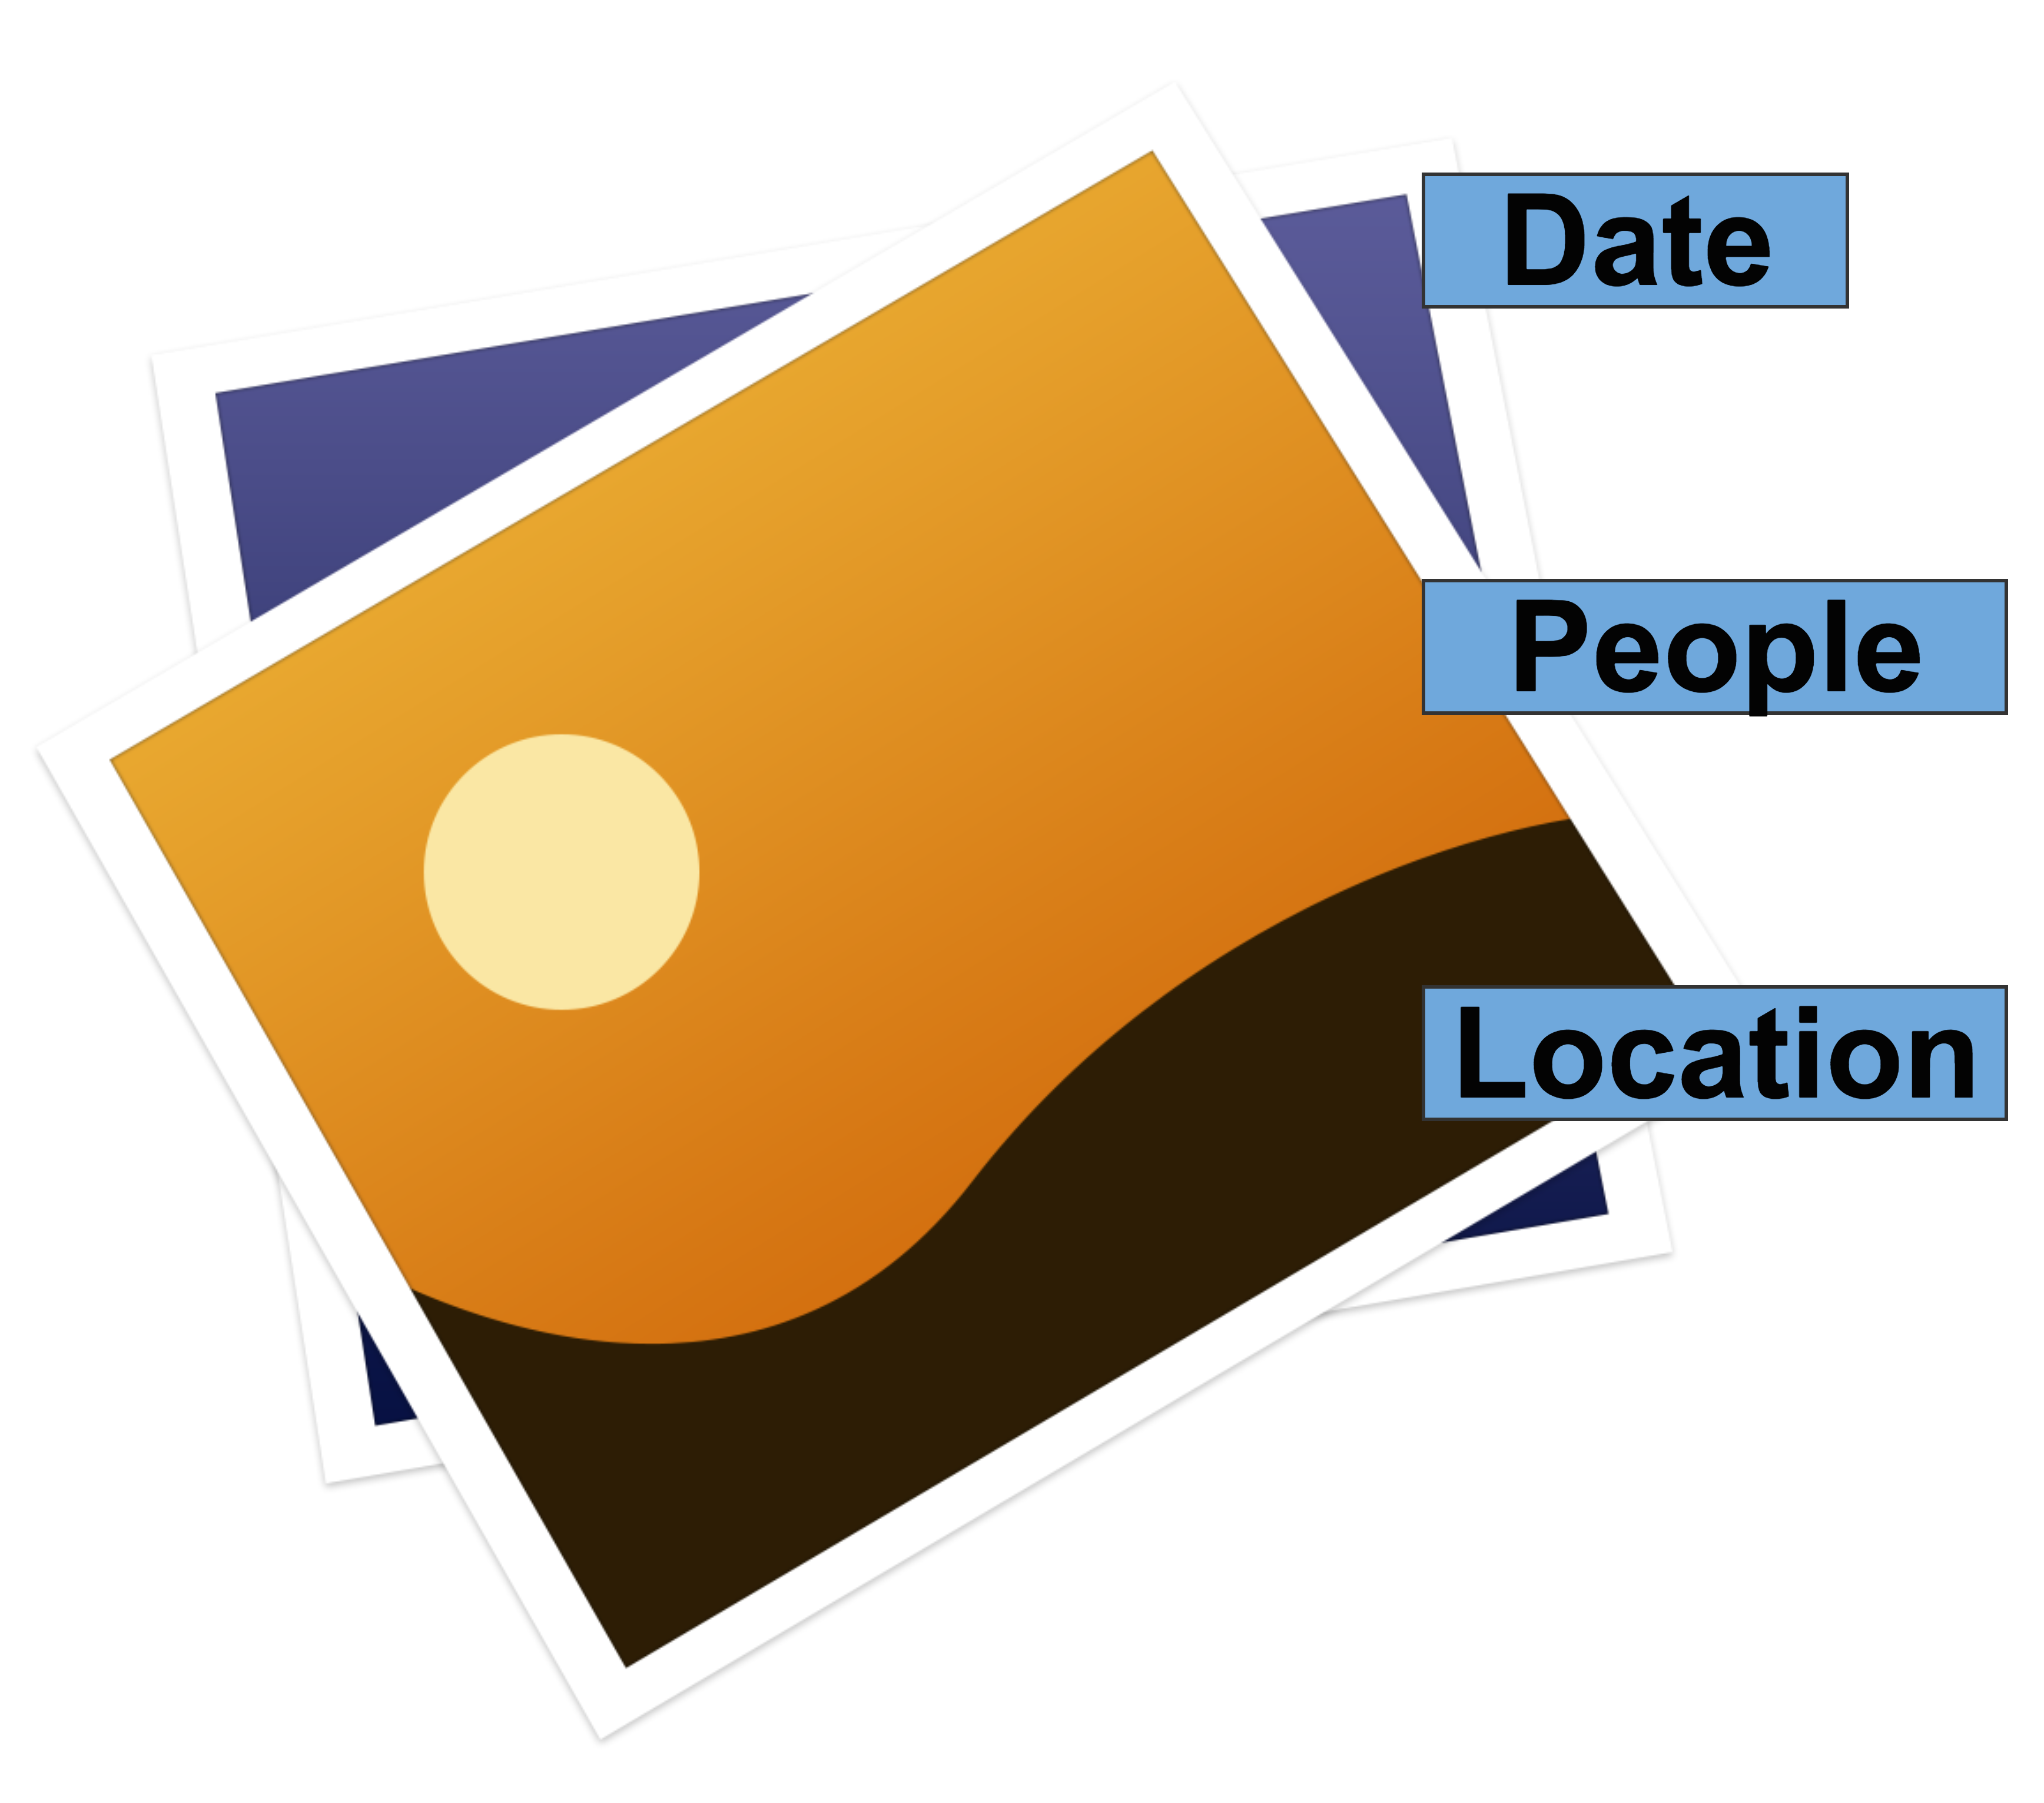
\includegraphics[width=0.7\textwidth]{images/slides/meta_image.png}
        \end{figure}
      \end{columns}

    \end{frame}

    \begin{frame}{Real World Applications}

      \begin{figure}
        \text{Google Query By Image}\par\medskip
        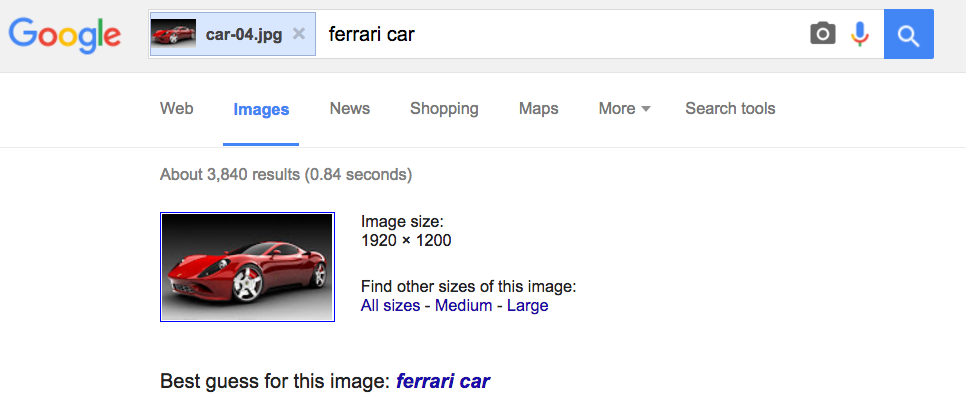
\includegraphics[scale=0.3]{images/slides/google_query_image.png}
      \end{figure}

    \end{frame}

    \begin{frame}{Real World Applications}

      \begin{columns}[c]
        \column{.5\textwidth} % column designated by a command
          \begin{center}
            CamFind
          \end{center}
          \begin{center}
            \begin{itemize}
              \item Entity Recognition
              \item Visual search engine
            \end{itemize}
          \end{center}
        \column{.5\textwidth}
        \begin{figure}
          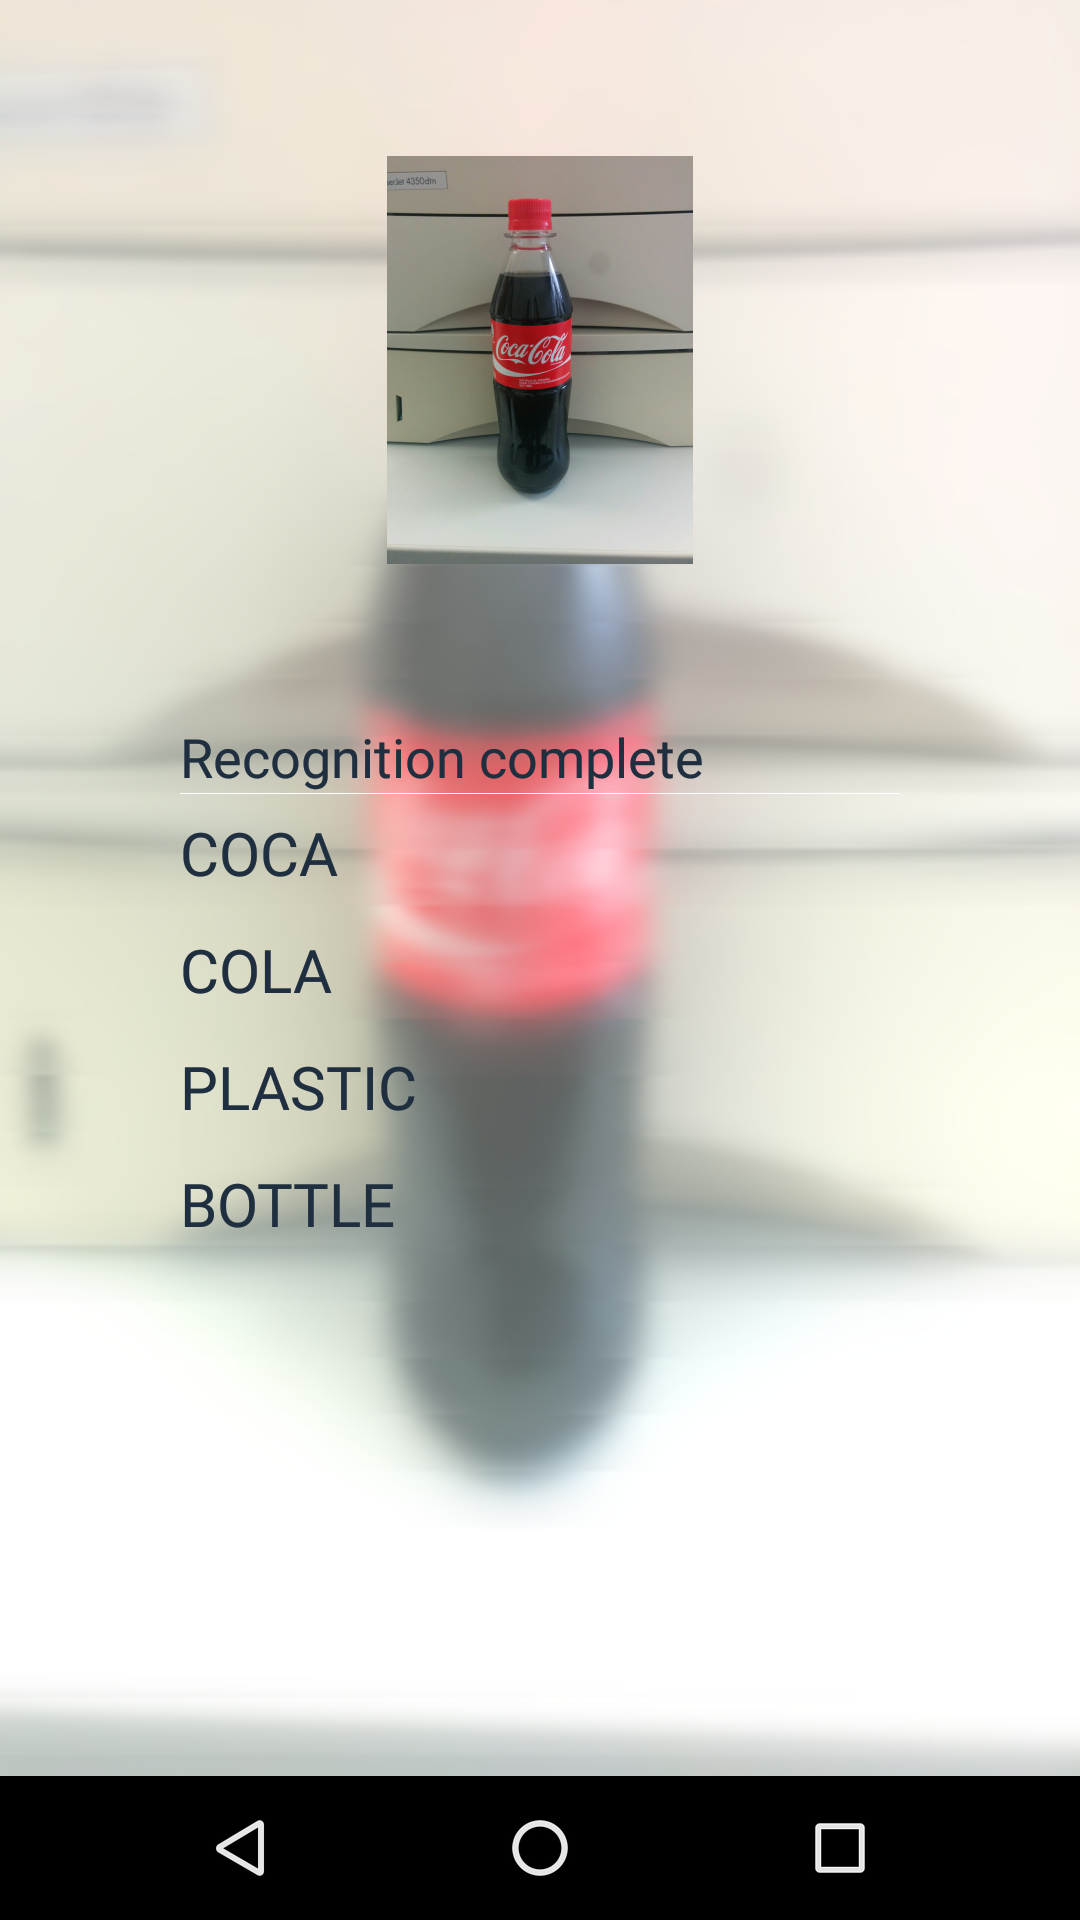
\includegraphics[width=0.6\textwidth]{images/slides/cam_find_1.png}
        \end{figure}
      \end{columns}

    \end{frame}

    \subsection{High level Pipeline}

    \begin{frame}{Pipeline}

        \begin{figure}
          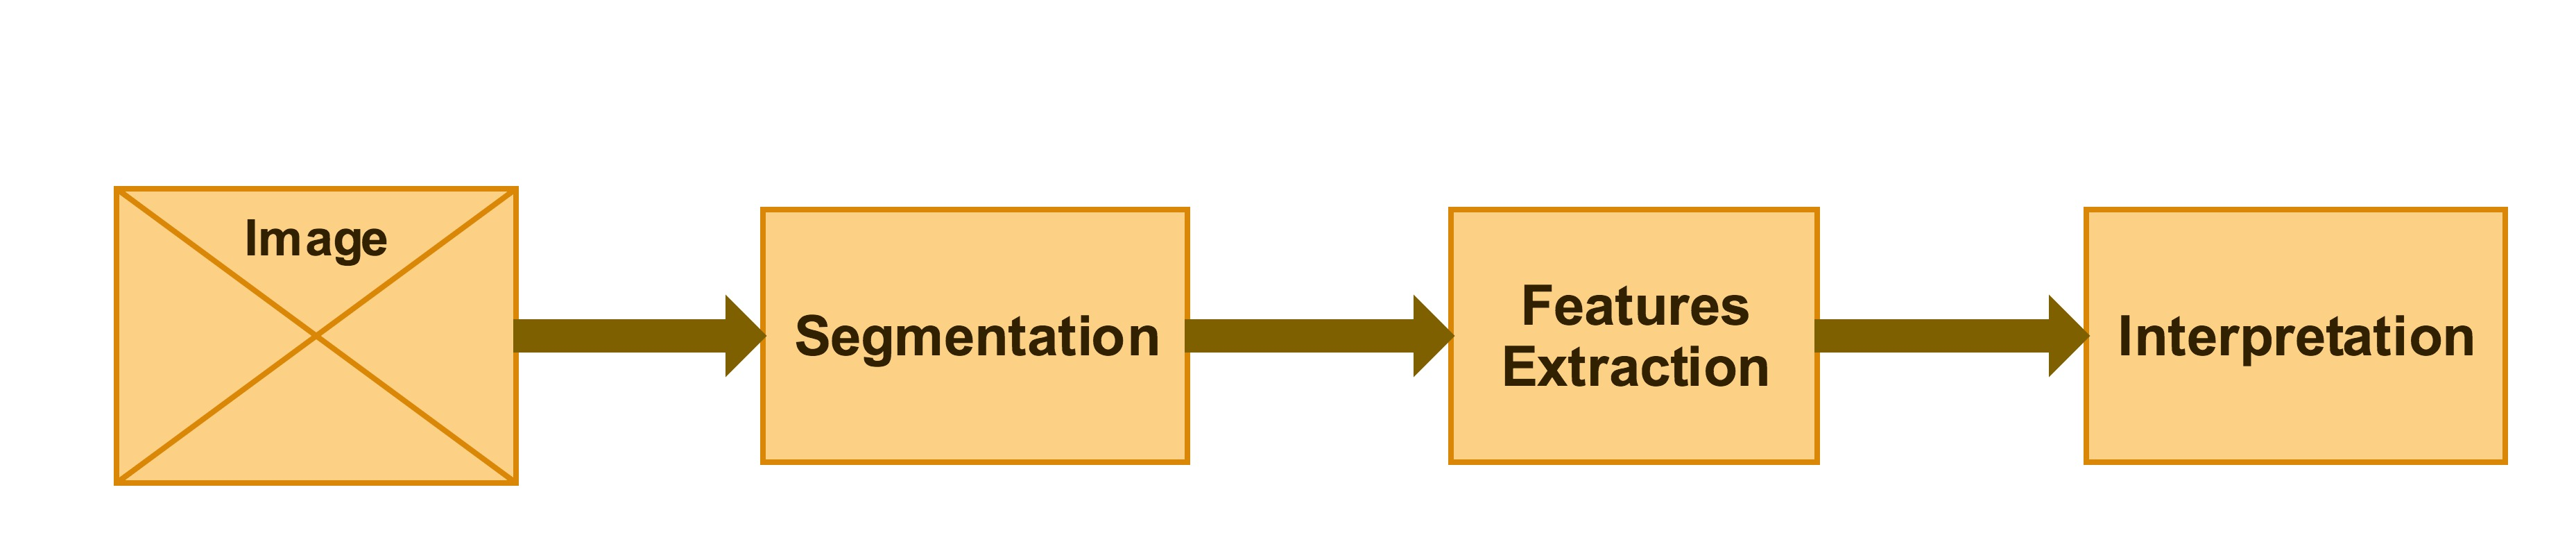
\includegraphics[width=1\textwidth]{images/slides/flow.jpg}
        \end{figure}

        \begin{center}
          Problems :
        \end{center}

        \begin{itemize}
          \centering
          \item A lot of different Features Detectors
          \item Low level Features
          \item Semantic Gap
        \end{itemize}

    \end{frame}

  \subsection{Research question}
    \begin{frame}{Research question}

      \begin{block}{The Semantic Gap}
        How deep learning methods can help to bridge the semantic gap in Content-Based Image Retrieval ?
      \end{block}

    \end{frame}

  \section{Research Trends}

    % \subsection{Deep Learning}
    %
    % \begin{frame}{Deep Learning}
    %
    %   \begin{center}
    %     \begin{itemize}
    %       \setlength\itemsep{1em}
    %       \item Much Deeper Architecture
    %       \item Higher Level Features
    %       \item No domain knowledge required
    %     \end{itemize}
    %   \end{center}
    %
    % \end{frame}


    \subsection{Convolutional Neural Network}

    \begin{frame}{Convolutional Neural Network}

      \begin{center}
        \begin{itemize}
          \setlength\itemsep{1em}
          \item Deep Learning method
          \item Learn Features from all kind of Signals
          \item Learn Higher Level Features
          \item Invariance to Several Transformations
        \end{itemize}
      \end{center}

    \end{frame}

    \subsection{Global Design}

    \begin{frame}{High Level Design}
      \begin{figure}
        \text{Design}\par\medskip
        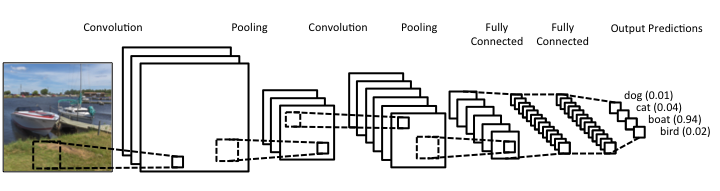
\includegraphics[scale=0.45]{images/slides/cnn_design.png}
      \end{figure}
    \end{frame}

    \subsection{Image Classification}

    \begin{frame}{LeNet-5 Breakthrough}

      \begin{columns}[c]

      \column{.5\textwidth}

          \begin{figure}
            \text{Handwritten Digit Recognition}\par\medskip
            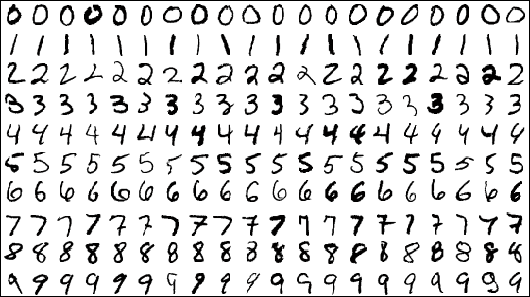
\includegraphics[width=0.6\textwidth]{images/slides/mnist.png}
          \end{figure}

      \column{.5\textwidth}

        \begin{center}
          Best Performance by LeNet 5 designed by Yann LeCun
        \end{center}
        \begin{itemize}
          \item Two Convolutional Layers
          \item One Fully Connected Layer
          \item One Softmax Layer
        \end{itemize}

      \end{columns}

      \end{frame}

  \begin{frame}{AlexNet Breakthrough}

    \begin{columns}[c]

      \column{0.5\textwidth}

        \begin{figure}
          \text{Image Classification}\par\medskip
          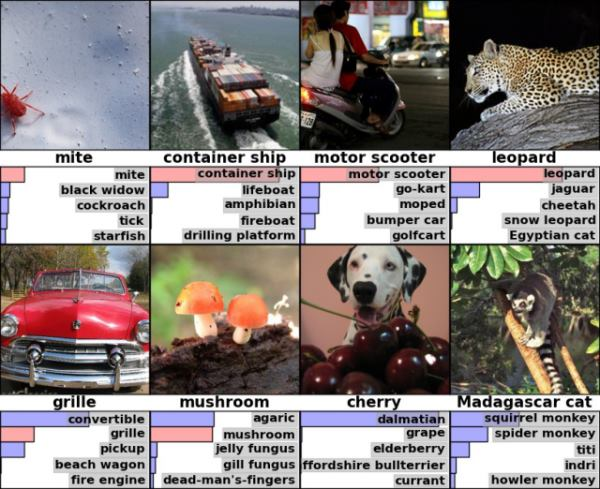
\includegraphics[width=0.6\textwidth]{images/slides/imagenet.jpg}
        \end{figure}

      \column{0.5\textwidth}

        \begin{center}
          Best Performance by AlexNet designed by Alex Krizhevsky
        \end{center}
        \begin{itemize}
          \item Five Convolutional Layers
          \item Three Pooling Layers
          \item Two Fully Connected Layers
          \item One Softmax Layer
        \end{itemize}

      \end{columns}

  \end{frame}

  \subsection{Image Similarity}

    \begin{frame}{Two Approaches}

      \begin{columns}[c]

        \column{.5\textwidth}
        \begin{figure}
          \text{Conventional}\par\medskip
          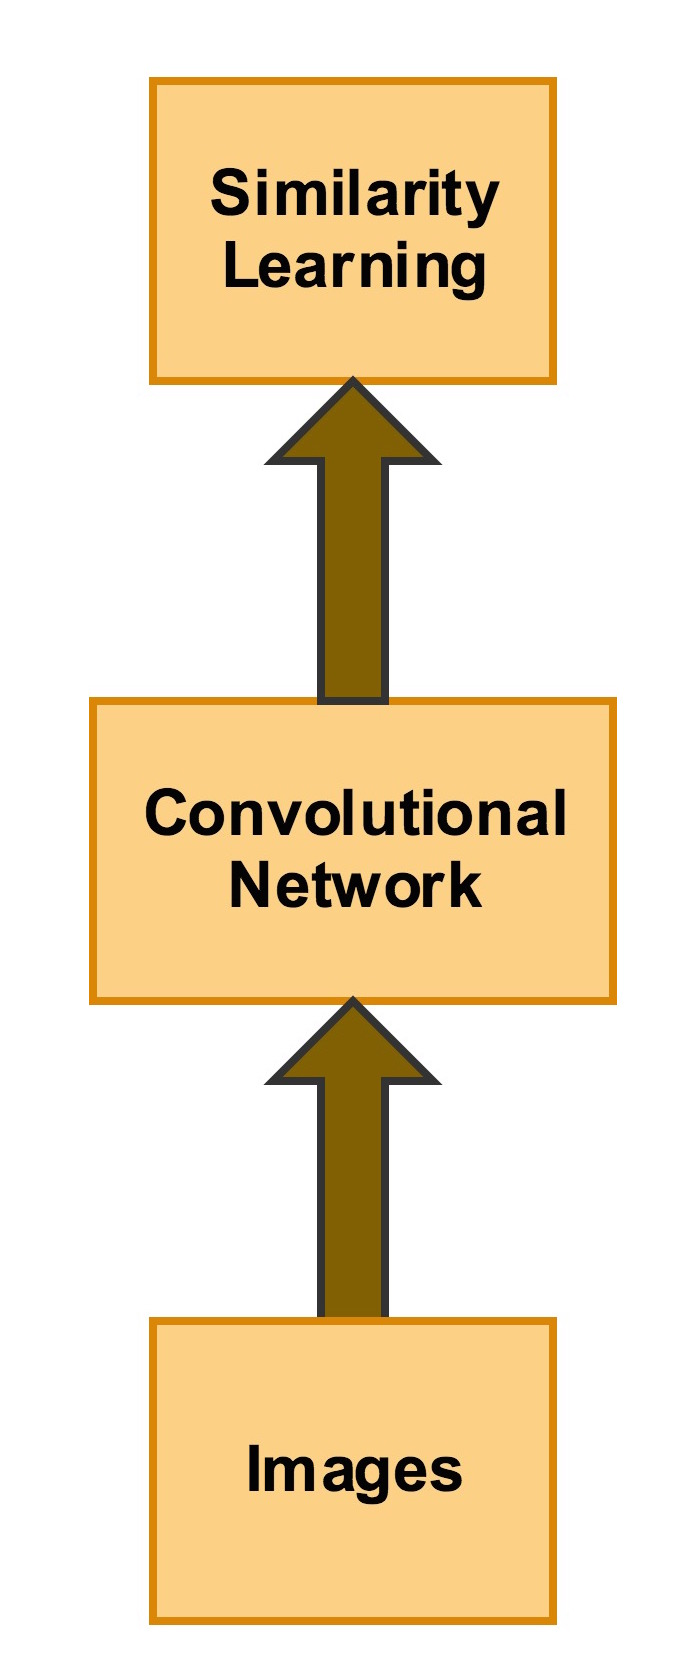
\includegraphics[width=0.45\textwidth]{images/slides/app.jpg}
        \end{figure}

        \column{.5\textwidth}
          \begin{figure}
            \text{Siamese Network}\par\medskip
            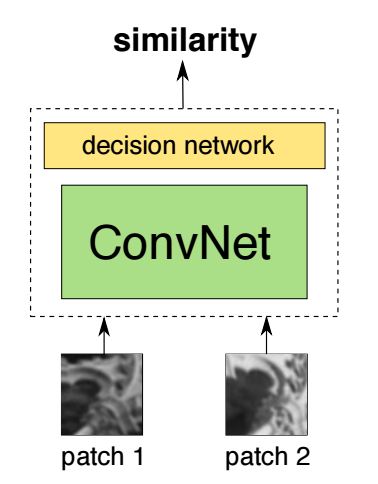
\includegraphics[scale=0.28]{images/slides/cnn2}
          \end{figure}

      \end{columns}
    \end{frame}

\section{My Work}

  \subsection{Objective}

  \begin{frame}{Objective}

    \begin{block}{Objective}
    Design a Convolutional Neural Network for Image Similarity Tasks.
    \end{block}

  \end{frame}

  \subsection{Roadmap}

  \begin{frame}{Roadmap}

    \begin{enumerate}
      \setlength\itemsep{1em}
      \item Re-implement traditional Convolutional Neural Network
      \item Design a new Convolutional Neural Network
      \item Evaluate the new net on several benchmarks
    \end{enumerate}
  \end{frame}

  \subsection{Implementation}

  \begin{frame}{Implementation}
    \begin{center}
      Deep Learning Framework Theano
    \end{center}

    \begin{itemize}
      \centering
      \setlength\itemsep{1em}
      \item Python library
      \item Implement a lot of useful functions
      \item Support GPU computing
    \end{itemize}
  \end{frame}

  \subsection{Evaluation}

  \begin{frame}{Evaluation}

    \begin{center}
      Three Benchmarks :
    \end{center}
    \begin{columns}[c]
      \column{.33\textwidth} % column designated by a command
      \begin{figure}
        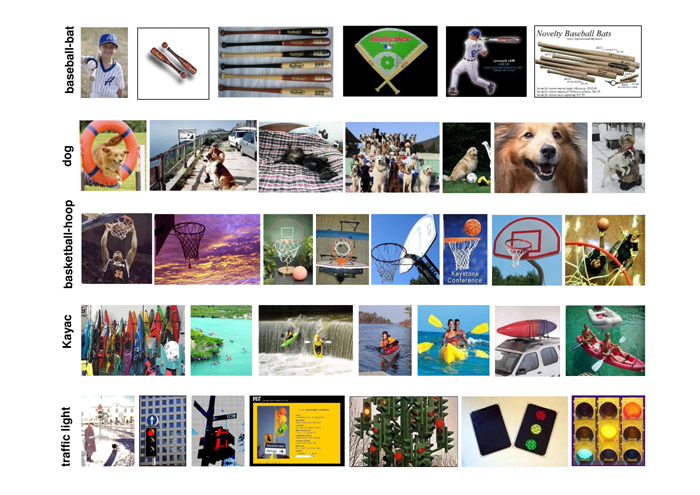
\includegraphics[width=0.6\textwidth]{images/slides/caldech256.jpg}
        \caption{Caldech}
      \end{figure}
      \column{.33\textwidth}
      \begin{figure}
        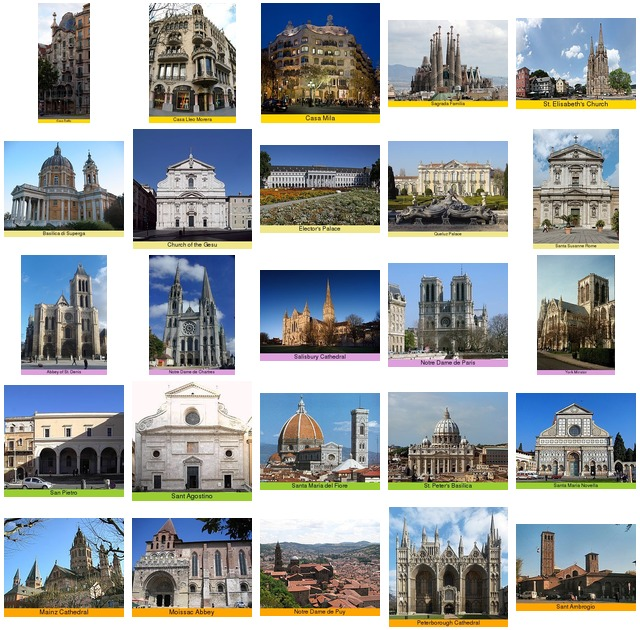
\includegraphics[width=0.7\textwidth]{images/slides/paris.jpg}
        \caption{Paris}
      \end{figure}
      \column{.33\textwidth}
      \begin{figure}
        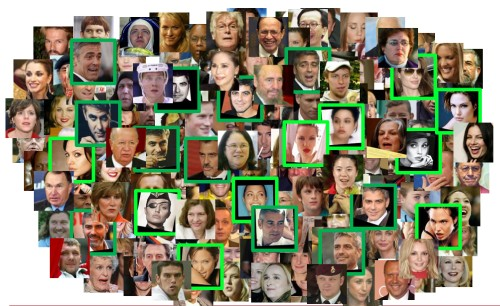
\includegraphics[width=0.7\textwidth]{images/slides/public.jpg}
        \caption{PubFig83}
      \end{figure}
    \end{columns}
\end{frame}

\section*{Summary}

\begin{frame}{Summary}

  % Keep the summary *very short*.
  \begin{itemize}
    \setlength\itemsep{1em}
  \item
    Content-Based Image Retrieval technologies are needed
  \item
    Convolutional Neural Network has already proven to be efficient for Image Classification
  \item
    Investigate how they can be used for Image Similarity
  \end{itemize}

\end{frame}

\begin{frame}
  \begin{center}
  Thank you for your attention !
\end{center}

\begin{center}
  Questions ?
\end{center}
\end{frame}



\end{document}
